% Be sure to write chapter titles in ALL CAPS
\chapter{\uppercase{EXPERIMENTS}}

\section{Research Questions}
There are four main questions of focus that the following experiments attempt to answer:
\begin{enumerate}
	\item What is the impact on the size of the test suite using abstract URLs instead of an exhaustive enumeration of every variable combination?
	\item What is the fault finding effectiveness of testing with abstract URLs versus exhaustive testing?
	\item What is the impact on the size of the test suite using combinatorial coverage compared to single coverage?
	\item What is the fault finding effectiveness of the combinatorial coverage compared with single coverage?
\end{enumerate}

\section{Sample Application}
All experiments were conducted on a sample Rich Web Application written by the author and is available at \url{http://chadmaughan.com/thesis}.  The application provides United States census information for 1990, 2000, and preliminary numbers from 2005 for each state, county, and city with a population over 25,000 residents.  The application is designed for mobile devices with larger touch points.  The sample application uses the following technologies:

\begin{enumerate}
\item Backbone.js: A client-side, JavaScript MVC framework that gives structure to rich web applications.  Backbone.js allows you to bind custom events to models, and route URL fragments to JavaScript functions.
\item jQuery Mobile: A unified, HTML5-based cross-platform user interface system for mobile devices.  It focuses on semantic markup that is easily themeable.
\item Spring MVC: A module of the popular Spring Framework for Java that allows for easy implementation of server-side controllers for building REST APIs.
\item Apache Derby DB: An open source, embedded relational database implemented in Java.
\end{enumerate}

Source code for both the application and the fault finding, testing code is also available at \url{http://code.chadmaughan.com/thesis}.  Metrics about the sample application are included in Table~\ref{table:sampleAppInfo}.  A sample screenshot of the application is provided in Figure~\ref{fig:screenshot}.

\begin{table}[h]
	\centering
	\caption{Sample Rich Web Application Information.}
	\begin{tabular}{| l | r|}
		\hline
Number of Application States		& 199,484 	\\ \hline
Number of Files				& 328 		\\ \hline
JavaScript Lines of Code			& 605 		\\ \hline
Java Number of Classes			& 21 		\\ \hline
Java Lines of Code				& 1,091 		\\ \hline
Seeded Faults					& 73 		\\ \hline
	\end{tabular}
\label{table:sampleAppInfo}
\end{table}

\begin{figure}[htbp]
\centering
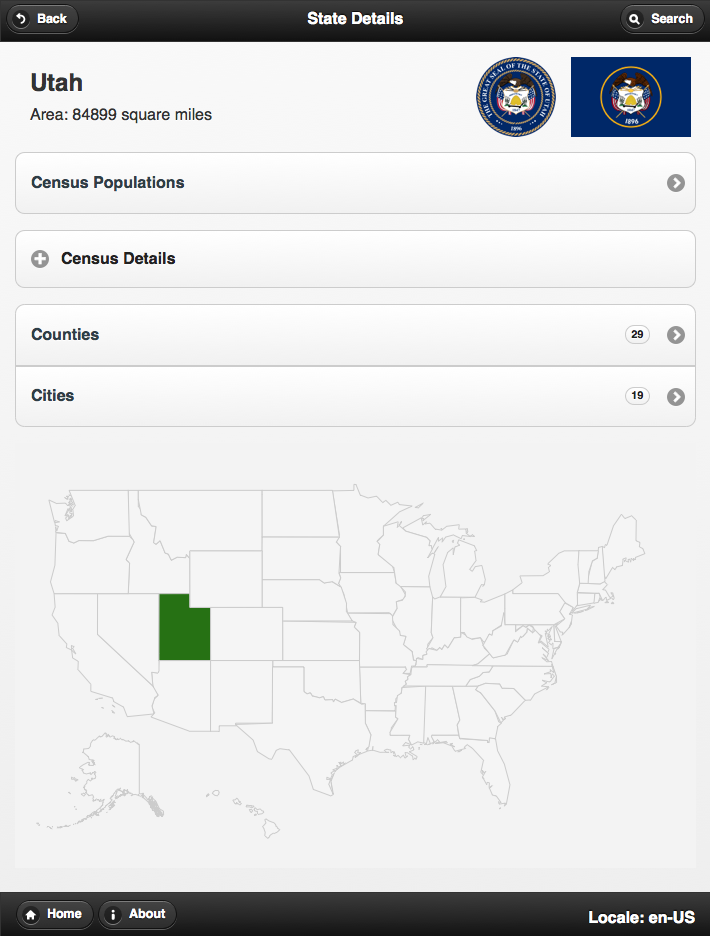
\includegraphics[width=0.9\textwidth]{images/ipad-screenshot.png}
\caption{Sample rich web application screenshot.}
\label{fig:screenshot}
\end{figure}

\section{JavaScript Faults}
The sample application is seeded with 73 faults.  A detailed list of those exceptions and the categories they belong to are listed in Table~\ref{table:seededExceptions}.  

On fault categories, Sampath et al. described five web application fault categories\cite{sampath2007applying}, of which all are used in the sample application.

\begin{enumerate}
\item Data store faults: Faults in the application code that manipulates data in any kind of data store.  This category of faults also applies to data that is incorrectly persisted in the data store.  There are a number of seeded data store faults in the sample application.

\item Logic faults: Faults in the application code that implements business logic and control flow.  An example of this is an error in the page transition with jQuery Mobile. 

\item Form faults: Faults in the application code that controls, modifies and displays name-value pairs in forms.  The sample application does not submit any data to the server but does use dynamically updated forms to direct to different application states.

\item Appearance Faults: faults in the application code that controls the way in which a web page is displayed.  With the use of modern JavaScript based templating solutions, such as Mustache.js and Underscore.js, appearance faults typically cause a template to not be rendered.  The sample application demonstrates this type of error when trying to load the search page.

\item Link faults: Faults in the application code that changes the page pointed to by an URL.
\end{enumerate}

Guo and Sampath \cite{guo2008web} add a sixth category, compatibility faults or ``faults in application code that ensures that the web application complies with different browsers, versions of browsers and other client environments.''  With the rapid introduction of new HTML5 APIs (i.e., Websockets and Webstorage) and the varying speed of adoption among browser creators, compatibility faults will play an increasingly important role in client-side testing.  

Guo also expands the logic faults category to include seven sub-categories.  The sub-categories of logic faults are:

\begin{enumerate}
\item Browser interaction faults: Faults in the application code that control the web browser, such as code that disables the ``back'' button on the browser, or code that is affected by user-defined browser settings, such as disabled cookies.  Browser manipulation is discouraged as it alters expected application behavior.  Other browser settings, such as disabling JavaScript, would render the application useless.  As such, the sample application does not use this fault sub-category.

\item Session faults: Faults in the application code that deal with maintaining state of application or other session-based operations such as using sessions to save and data entered into a form and display the data after the sessions has been validated.  As most rich web applications are stateless to avoid the overhead of session management and allow for greater scalability, the sample application does not use this sub-category.

\item Paging faults: Faults in the application code that deals with paging when displaying large amounts of data on the screen.  While applicable to rich web applications, the sample application does not use this sub-category.

\item Server-side parsing faults: Faults in the application code that deal with server-side parsing of HTML, XML, and JavaScript tags.  This sub-category does not apply to rich web applications as HTML used in a RWA is typically a minimal page used only as an entry point.  ``client-side parsing faults''  are more applicable to rich web applications.   The sample application has a number JavaScript syntax related faults.  These errors are described below in Table~\ref{table:seededExceptions}.

\item Encoding/decoding faults: Faults in the application code that encodes or decodes characters for transmission, storage, and display

\item Locale faults: Faults that exist in application code that sets or gets locale-specific information, such as date format or language.  Not used in the sample application.

\item Other: Other logic faults that do not belong to any of the above sub categories.
\end{enumerate}

More recently, in addition to Sampath and Guo, Ocariza et al. \cite{ocariza2011javascript} defines five categories specifically for JavaScript exceptions.  He found that JavaScript exceptions tend to be much more defined than other applications and fall into well-defined categories.  In fact, 94\% of all errors studied from the Alexa top 100 list fall into five categories, namely:

\begin{enumerate}
\item Permission Denied:  Faults in the application code that attempt to access JavaScript components from another domain violating the same-origin policy.  The sample application has a seeded fault where it tries to load recent search data from Twitter and violates the same-origin policy. 

\item Null Exception faults: Faults in the application code where a property or method is accessed via a null object.  The sample application attempts to add a CSS class name to an element that is null.

\item Undefined Symbol faults: Faults in the application code where a function or variable is accessed that has not been previously defined.

\item Syntax Error faults: Faults in the application code where interpreted code, such as in an eval() function, has the wrong syntax.

\item Miscellaneous faults: Faults in the application code that apply specifically to a single site.
\end{enumerate}

These five categories align more closely with the JavaScript Error object and its six other core errors: EvalError (Syntax Error faults), RangeError, ReferenceError (Undefined Symbol faults), SyntaxError (Syntax Error faults), TypeError, and URIError\cite{mdnError}.

\begin{table}[h]
	\centering
	\caption{Sample Rich Web Application Seeded Errors.}
	\begin{tabular}{| l | p{5cm} | p{3cm} | l |}
		\hline

Location    &    Description    &    Category    &    Count		\\ \hline

index.html:39 	&
console.log(variable) - variable is not defined.  & 
ReferenceError, Undefined& 
1 
\\ \hline

main.js:54	& 
SearchPageView template is not included as a source.  & 
ReferenceError, Appearance&
1 
\\ \hline

geochart:438& 
County Map doesn't exist on County Details page. "Container is not defined" error.  & 
Appearance& 
1 (3,144)
\\ \hline

main.js:49&
Syntax Error on eval() - eval("window.print(;") & 
SyntaxError & 
1 
\\ \hline

main.js:37& 
Missing script file - notthere.js"  & 
Link, Other, Misc& 
1 
\\ \hline

jquery-1.7.1.min.js:4 & 
Multiple words in the name (9 states plus Washington DC) doesn't have a flag to display & 
& 
10 
\\ \hline

jquery-1.7.1.min.js:4 & 
Multiple words in the name (9 states plus Washington DC) doesn't have a seal to display & 
Appearance& 
10 
\\ \hline

CityController.java:39&
Cities with periods in their name/code, return HTTP 500 (i.e., St. George, UT). & 
Data Store & 
13 
\\ \hline

index.html:87& 
Type Error 'bad type' for all Washington State cities & 
TypeError, Misc& 
37 
\\ \hline

twitter.js:4& 
City Twitter Search feed & 
Permission & 
1 (1,267)
\\ \hline

census-table-view.js:17& 
Adds a CSS class to a null element& 
Null Exception, TypeError & 
1
\\ \hline

	\end{tabular}
\label{table:seededExceptions}
\end{table}

\section{Testing Technologies}
In addition to the sample Rich Web Application, the code used to identify the seeded faults rely on some key technologies.  These technologies are listed below:

\begin{enumerate}
\item Neo4j: A powerful graph database with a rich API that was used to both systematically identify variables in semantic URLs and store a full navigation graph of the rich web application for test traversal retrieval.

\item BrowserMob: An embedded proxy software that allows the interception of HTTP requests from the client and HTTP responses from the server.  This allows for the identification of network errors and for the modification of the server responses to assist in identifying client side JavaScript errors.

\item Selenium WebDriver: Allows for the crawling and interaction with the application in the various browsers ``as the user would,'' giving a more accurate result while testing.
\end{enumerate}

\section{Navigation Graph}
A navigation graph is a visual representation of an application\cite{herman2000graph}.  A navigation graph of a rich web application is a visual representation of how different states of the web application are related to one another.  A traditional web application navigation graph typically would have a single node for each HTML page or a single node for each rendering of a server-side script.  An edge on a traditional web application represents an HTML anchor tag.  As rich web applications typically have a single or very limited number of HTML pages acting as entry points, a node in the navigation graph of a rich web application represents a single state of the application.  An edge in a navigation graph for a rich web application represents a transition from one state to another.  Like in a traditional web application, this is also typically done through an HTML anchor tag.

Building a navigation graph of the rich web applications has many benefits, including understanding the application as a whole, maintenance over the development cycle, and test case generation and the subsequent testing of those tests\cite{wang09}.  To build the graph, and expand it as the application increases in size, a rich web application can be crawled using the Selenium WebDriver in a simple depth first traversal.  Figure~\ref{crawlingAlgorithm} demonstrates the crawling algorithm using Selenium WebDriver.

\begin{figure}
\begin{lstlisting}
	public static void main(String[] args) {
		driver = new FirefoxDriver();
		new Crawl("http://example.com");
	}

	public Crawl(String startingUrl) throws Exception {
		String newAddress = null;
		while ((newAddress = queue.poll()) != null)
			processPage(newAddress);
	}

	private void processPage(String sourceHref) throws Exception {
		driver.get(sourceHref);
		List<WebElement> links = driver.findElements(By.tagName("a"));
		Node sourceNode = retrieveOrCreateNode(sourceHref);
		String targetHref;

		for (int i = 0; i < links.size(); i++) {
			WebElement w = links.get(i);		
			targetHref = w.getAttribute("href");
			if (isValidUrl(targetHref)) {
				if(w.isDisplayed()) {
					Node targetNode = retrieveOrCreateNode(targetHref);				
					if(targetNode == null)
						targetNode = nodeMapper.mapNode(targetHref, w);				
					sourceNode.createRelationshipTo(targetNode, 
							RelationshipTypes.LINKS_TO);
					if (!processed.contains(targetHref))
						queue.add(targetHref);
				}
			}
		}
	}
\end{lstlisting}
\caption{Depth first crawling of a rich web application}
\label{crawlingAlgorithm}
\end{figure}

Also of benefit is the ability to identify key, holistic characteristics about the application as the navigation graph is built.  For example, while this experiment does not focus on test prioritization, systematically creating a navigation graph with Selenium WebDriver allows you to easily record and track key information about state transitions in the application.  As an example, one may wish to prioritize testing based on the location of links or elements that trigger a change in state.  Combining the exact top and left pixel location of that element allows you to prioritize links that are more in the key navigation sections.  As another prioritization strategy with a navigation graph, one could also easily prioritize based on states of the application that are most transitioned.

\section{Abstract URLs}
One problem with the depth-first traversal of a rich web application is the time it takes to complete a full application crawl.  For example, the sample census application discussed previously contains nearly 200,000 different states.  Assuming an average page load of around 500 milliseconds, it would still require more than 27 hours to perform a full regression test.  While this amount of time to perform an exhaustive regression test is possible, it may not always be practical.

Using variables previously identified through the algorithm described in the background chapter, application states can be stored in the navigation graph as ``abstract URLs''\cite{wang09}, or URLs with variable names instead of each possible value.  Similar to semantic URL formats discussed earlier, an example of an abstract semantic URL stored in a navigation graph would look as follows:

\begin{figure}[H]
\centering
http://example.com/\#/state/\{var1\}/county/\{var2\}/city/\{var3\}
\end{figure}

Storing the abstract URL instead of every URL variable combination significantly reduces the number of tests required.  Indeed, it is ideal as most rich web application states reuse small HTML templates for the displaying of particular data points.  This means that client-side errors would typically manifest themselves for every variance of a variable.  One disadvantage of using abstract URLs is that data specific errors may be missed.  For example, the sample application has a fault where any city with a period in it's name (i.e., ``St. George, UT'') doesn't render correctly.  Unless the random value for the abstract URL variable selected contained a period, this data related fault would be missed.  While not discussed in detail in this paper, due to the available resource of the full application structure (from the systemic variable identification), one possibility is to use a sample size confidence level to adequately test a certain size of the data available.

One of the experiments completed was calculating and comparing the amount of time required to crawl a full rich web application, a reduced number of states based on a sample size, and a fully reduced test suite testing only abstract URLs one time.  Results of this experiment are discussed in the following chapter.

\section{Capturing Errors}
Another difficulty encountered with testing rich web applications is the ability to identify errors that occur in the browser.  JavaScript errors are difficult to systematically intercept and report.  This section introduces a novel approach for identifying two different types of exceptions during testing, namely network related and JavaScript browser related.

Some network related exceptions are errors that are simple to identify on the server-side by examining the log files.  BrowserMob was used as an embedded proxy to intercept all communications between the browser and the server.  This allows for the logging of network related exceptions, as well as response interception and subsequent modification for JavaScript exception reporting.

JavaScript exceptions in modern browsers typically manifest themselves via the browser console object.  The console is typically not visible to the end user and needs to be enabled via menu options or browser plug-ins such as Firebug for Firefox.  A sample of thrown exception is shown in Figure~\ref{fig:consoleError}.

\begin{figure}[H]
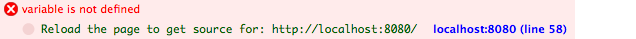
\includegraphics[width=0.9\textwidth]{images/console-error.png}
\caption{An example JavaScript error in the Firebug console.}
\label{fig:consoleError}
\end{figure}

Unfortunately, once these exceptions are thrown, there is no way to retrieve them from the browser.  A simple way to capture these is to introduce a small snippet of JavaScript code in every HTML entry point that has a collection for inserting exceptions.  This requires that testing code be added to the deployable deliverable, considered by many to be bad practice.  As an alternative, this experiment introduces a novel approach to keep testing scaffolding out of the deployable code base.  BrowserMob is used in to intercept only full HTML page responses from the server to the browser, and alter it injecting a custom browser Console object at the beginning of the HTML \textless script\textgreater\  tag.  This custom Console object stores any exception for later retrieval and reporting.  Figure~\ref{consoleJavascript} shows the custom JavaScript injected into each response.

\begin{figure}
\begin{lstlisting}[language=HTML]
	<script type="text/javascript">
		window.jsErrors = [];
		window.onerror = function(errorMessage) {
			window.jsErrors[window.jsErrors.length] = errorMessage;
		}
	</script>
\end{lstlisting}
\caption{Browser exception catching}
\label{consoleJavascript}
\end{figure}

\section{Combinatorial Testing}
The preparation done with the creation of both the exhaustive and the reduced navigation graph has prepared for the generation of combinatorial test cases.  The sample application has some variables, namely state, county, and city, that are hierarchical in nature.  Czerwonka\cite{czerwonka2008pairwise}, while describing the capabilities of the Microsoft PICT combinatorial test generation tool, explains that these hierarchical variables are treated as a ``sub-model'' and pairwise combined first to represent a single variable that is then used in the generation of the combinatorial test cases.  For example, in the sample application on the home page, the State of Utah, Cache County, and Logan City are combined together to form a single variable that is then used in building the combinatorial tests.  Additionally, a great majority of exceptions that occur in rich web applications result from the different browsers and environments.  Tatsumi\cite{grochtmann1995test} made the distinction of input and environment variables.  The input variables discovered via the process introduced previously can then be combined with provided environment variables to also identify ``compatibility faults.''  I discuss in the concluding chapter future work that can add distributed computing capabilities enabling browsers in different client environments to perform the same tests.